\documentclass[12pt,]{article}
\usepackage[superscript,nomove]{cite} % use if \cite is used and superscripts wanted
\usepackage[utf8]{inputenc}
\usepackage[a4paper, margin=1.2in]{geometry}
\usepackage{amsmath}
\usepackage{graphicx}
\usepackage{lscape}
\usepackage{bbm}
\usepackage{mathrsfs}
\usepackage{amssymb}
\usepackage{amsmath,amssymb,amsthm}
\usepackage{listings}
\usepackage{color} %red, green, blue, yellow, cyan, magenta, black, white
\usepackage{longtable}
\usepackage{tabularx}
\usepackage{rotating}
\usepackage{fancyhdr}          % this and next line are for fancy headers/footers
\pagestyle{fancy}
\usepackage{float}

\usepackage{Sweavel}

% To produce both postscript and pdf graphics, remove the eps and pdf
% parameters in the next line.  Set default plot size to 6x4 in.

%\SweaveOpts{width=8, height=6}



\begin{document}
\begin{titlepage}
\begin{center}

\vspace*{5em}
{\huge Relative Efficiency of Pennsylvania Dairy Farms\\[0.4cm] }
\color{blue}\hrule
\color{black}
\vspace{100mm}
\noindent
\Large 
Robert D \textsc{Weaver}\\
and\\
Jiachuan \textsc{Tian}

\today
\vfill
\end{center}
\end{titlepage}



%--------------------------------
\section{Data Desciption}
%--------------------------------
In this note, we present an analysis of farms' production efficiencies using the DEA approach. The data we use is monthly data of a small set of Pennsylvania dairy farms. The data was collected from 53 farms that participated in the study. The three datasets can be summarized as:



% latex table generated in R 3.2.2 by xtable 1.8-2 package
% Fri Apr 01 23:40:07 2016
\begin{table}[ht]
\centering
\begin{tabularx}{\linewidth}{ll|l|X}
  \hline
 & Data\_set & Number\_obs & Comments \\ 
  \hline
1 & Monthly Data & 2303.00 & IOFC data collected for each month 2013-2015, 53 farms, test date data included \\ 
  2 & Test Data & 144.00 & Test dates pooled such that for each farm there are 3-5 obs on different test dates \\ 
  3 & Annual Data & 55.00 & 2013-2015 although 53 farms x 2yrs =$>$ 106 obs, many farms had missing data \\ 
   \hline
\end{tabularx}
\caption{Summary of Datasets} 
\label{Table-1}
\end{table}

%--------------------------------
\section{Models}
%--------------------------------
Now we define the input and output variables we use in the models. The inputs variates we choose are:
\begin{center}
Number of Cows, Dry Matter, CP, Starch DM, pH\\
Purchased Feed, Feed Cost, Corn silage\\
\end{center}
Note inputs in last row below are only in annual data.

The outputs variates we choose are:
\begin{center}
Milk per Milk Cow, Fat, Protein, (negative) MUN, (negative)Fecal Starch
\end{center}



\subsection{Model 4-1 Test Data}
Recall in test data, the test dates are pooled such that for each farm there are 3-5 obs on different test dates. For each of the output variables, we conduct DEA for all farms. The average efficiency scores can be summarized in table 2.

% latex table generated in R 3.2.2 by xtable 1.8-2 package
% Fri Apr 01 23:40:07 2016
\begin{longtable}{l|l|l|l|l|l|l}
  \hline
 & Farm\_ID & Milk\_per\_Milk\_Cow & X\_\_Fat & X\_\_Pro & MUN & Fecal\_Starch \\ 
  \hline
1 & 3.00 & 0.93 & 0.92 & 0.93 & 0.92 & 0.92 \\ 
  2 & 4.00 & 0.99 & 0.91 & 0.91 & 0.91 & 0.91 \\ 
  3 & 5.00 & 0.99 & 0.91 & 0.91 & 0.91 & 0.97 \\ 
  4 & 9.00 & 0.93 & 0.95 & 0.94 & 0.94 & 0.97 \\ 
  5 & 10.00 & 0.87 & 0.90 & 0.87 & 0.87 & 0.87 \\ 
  6 & 14.00 & 0.91 & 0.90 & 0.90 & 0.90 & 0.91 \\ 
  7 & 18.00 & 0.92 & 0.89 & 0.89 & 0.89 & 0.89 \\ 
  8 & 21.00 & 0.93 & 0.93 & 0.93 & 0.93 & 0.95 \\ 
  9 & 22.00 & 0.93 & 0.92 & 0.92 & 0.92 & 0.92 \\ 
  10 & 23.00 & 1.00 & 1.00 & 1.00 & 1.00 & 1.00 \\ 
  11 & 24.00 & 0.92 & 0.90 & 0.91 & 0.90 & 0.92 \\ 
  12 & 25.00 & 0.97 & 0.95 & 0.95 & 0.96 & 0.99 \\ 
  13 & 31.00 & 0.94 & 0.93 & 0.92 & 0.91 & 0.94 \\ 
  14 & 37.00 & 0.97 & 0.96 & 0.96 & 0.96 & 0.97 \\ 
  15 & 38.00 & 0.91 & 0.90 & 0.90 & 0.91 & 0.94 \\ 
  16 & 51.00 & 1.00 & 1.00 & 1.00 & 1.00 & 1.00 \\ 
  17 & 60.00 & 0.95 & 0.91 & 0.91 & 0.93 & 0.92 \\ 
  18 & 61.00 & 0.93 & 0.92 & 0.92 & 0.94 & 0.92 \\ 
  19 & 62.00 & 0.94 & 0.94 & 0.93 & 0.93 & 0.93 \\ 
  20 & 63.00 & 0.98 & 0.93 & 0.93 & 0.94 & 0.94 \\ 
  21 & 65.00 & 0.88 & 0.86 & 0.86 & 0.86 & 0.86 \\ 
  22 & 66.00 & 0.89 & 0.86 & 0.86 & 0.88 & 0.86 \\ 
  23 & 67.00 & 0.94 & 0.86 & 0.86 & 0.86 & 0.86 \\ 
  24 & 69.00 & 0.98 & 0.94 & 0.94 & 0.95 & 0.95 \\ 
  25 & 70.00 & 0.96 & 0.92 & 0.92 & 0.92 & 0.93 \\ 
  26 & 93.00 & 1.00 & 0.91 & 0.91 & 1.00 & 0.94 \\ 
  27 & 95.00 & 0.90 & 0.92 & 0.89 & 0.90 & 0.92 \\ 
  28 & 106.00 & 0.99 & 0.96 & 0.96 & 0.97 & 0.99 \\ 
  29 & 107.00 & 0.97 & 0.96 & 0.96 & 0.98 & 0.96 \\ 
  30 & 111.00 & 0.87 & 0.90 & 0.88 & 0.87 & 0.87 \\ 
  31 & 113.00 & 0.93 & 0.91 & 0.91 & 0.92 & 0.96 \\ 
  32 & 115.00 & 0.99 & 0.96 & 0.96 & 0.97 & 0.99 \\ 
  33 & 129.00 & 0.89 & 0.90 & 0.89 & 0.87 & 0.89 \\ 
  34 & 130.00 & 0.98 & 0.96 & 0.96 & 0.96 & 0.98 \\ 
  35 & 133.00 & 0.93 & 0.89 & 0.89 & 0.89 & 0.93 \\ 
  36 & 135.00 & 0.91 & 0.88 & 0.88 & 0.88 & 0.88 \\ 
  37 & 144.00 & 0.97 & 0.99 & 0.99 & 0.97 & 0.99 \\ 
  38 & 146.00 & 0.93 & 0.96 & 0.93 & 0.92 & 0.97 \\ 
  39 & 149.00 & 0.95 & 0.92 & 0.92 & 0.92 & 0.92 \\ 
  40 & 150.00 & 0.96 & 0.92 & 0.92 & 0.95 & 0.92 \\ 
  41 & 153.00 & 0.97 & 1.00 & 0.97 & 0.97 & 0.97 \\ 
  42 & 159.00 & 1.00 & 0.94 & 0.94 & 0.95 & 0.97 \\ 
  43 & 162.00 & 0.95 & 0.95 & 0.95 & 0.96 & 0.95 \\ 
  44 & 163.00 & 0.93 & 0.96 & 0.93 & 0.93 & 0.93 \\ 
  45 & 164.00 & 0.99 & 1.00 & 0.99 & 1.00 & 1.00 \\ 
  46 & 170.00 & 1.00 & 0.99 & 0.99 & 1.00 & 0.99 \\ 
  47 & 179.00 & 0.95 & 0.92 & 0.92 & 0.93 & 0.97 \\ 
  48 & 180.00 & 0.99 & 0.98 & 0.98 & 1.00 & 1.00 \\ 
  49 & 194.00 & 0.94 & 0.94 & 0.94 & 0.94 & 0.95 \\ 
  50 & 195.00 & 0.90 & 0.88 & 0.88 & 0.91 & 1.00 \\ 
  51 & 196.00 & 0.90 & 0.89 & 0.89 & 0.89 & 1.00 \\ 
  52 & 198.00 & 0.92 & 0.90 & 0.90 & 0.93 & 0.90 \\ 
   \hline
\hline
\caption{Average Test Data Efficiency Score by Farm} 
\label{Table-2}
\end{longtable}Each column is table 2 reports the average efficiency score based on that column as output. We plot the distribution of the efficiency scores in figure 1 and figure 2.

\begin{figure}[H]
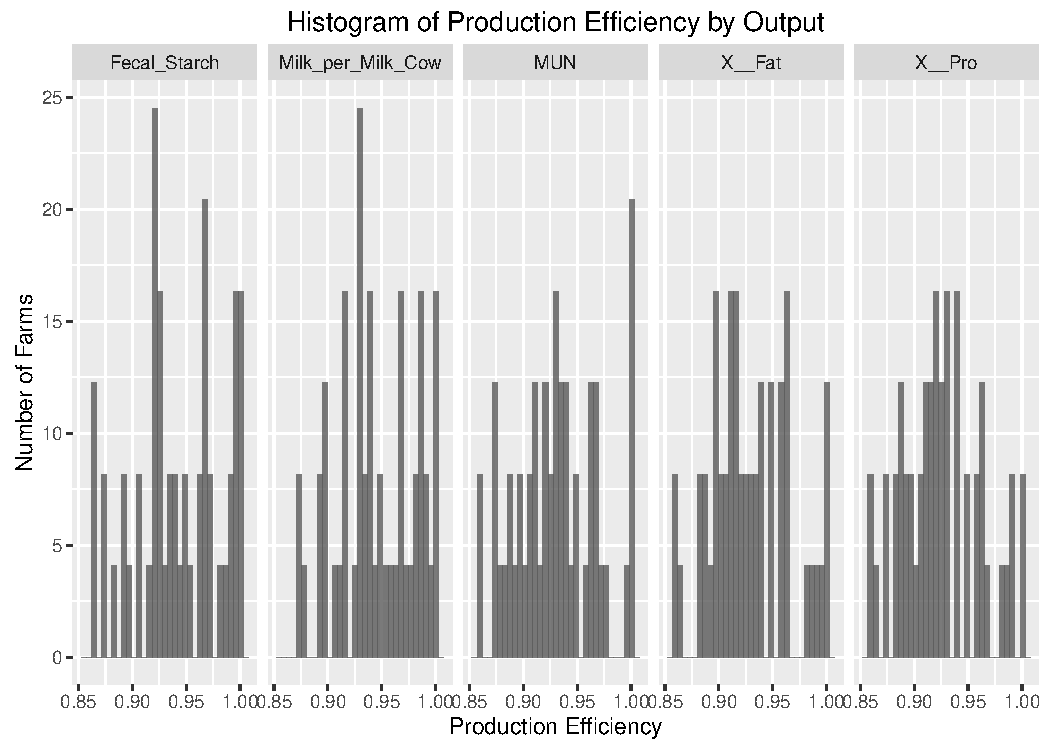
\includegraphics{Final_Model-11}
\caption{Histogram of Average Efficiency Score for each farm}
\end{figure}


\begin{figure}[H]
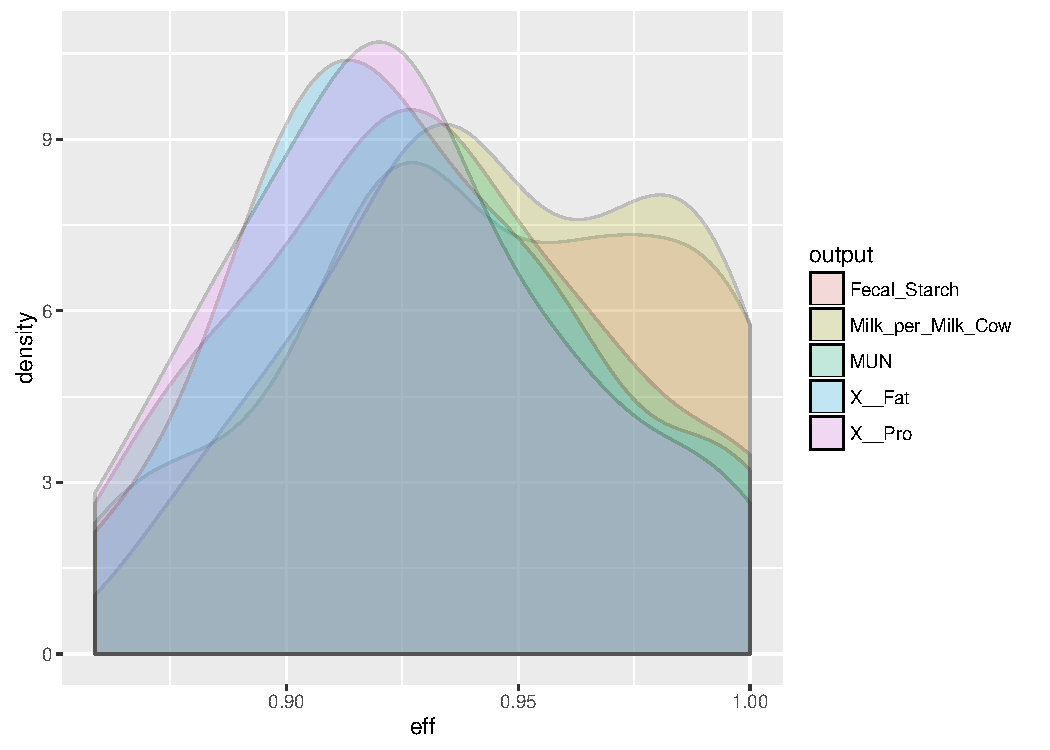
\includegraphics{Final_Model-22}
\caption{Distribution of Average Efficiency Score for each farm}
\end{figure}

\subsection{Model 4-2 Test Data Seperated}
In the section, we examine whether the efficiency of farms vary over time.  Thus we partition the test data based on test date. Each test date considered a different sample.

The efficiency scores are reported in table 3.
% latex table generated in R 3.2.2 by xtable 1.8-2 package
% Fri Apr 01 23:40:08 2016
\begin{longtable}{l|l|l|l|l|l|l|l}
  \hline
 & Farm\_ID & Season\_Year & Milk\_per\_Milk\_Cow & X\_\_Fat & X\_\_Pro & MUN & Fecal\_Starch \\ 
  \hline
1 & 3.00 & Fall 2013 & 0.93 & 0.93 & 0.94 & 0.93 & 0.93 \\ 
  2 & 3.00 & Spring 2014 & 0.94 & 0.92 & 0.92 & 0.92 & 0.92 \\ 
  3 & 3.00 & Spring 2015 & 1.00 & 1.00 & 1.00 & 1.00 & 1.00 \\ 
  4 & 3.00 & Fall 2015 & 1.00 & 1.00 & 1.00 & 1.00 & 1.00 \\ 
  5 & 4.00 & Fall 2013 & 1.00 & 0.96 & 0.96 & 0.96 & 0.96 \\ 
  6 & 4.00 & Spring 2014 & 1.00 & 0.92 & 0.92 & 0.92 & 0.92 \\ 
  7 & 4.00 & Fall 2014 & 1.00 & 1.00 & 1.00 & 1.00 & 1.00 \\ 
  8 & 5.00 & Fall 2013 & 1.00 & 1.00 & 1.00 & 1.00 & 1.00 \\ 
  9 & 5.00 & Fall 2014 & 0.99 & 0.94 & 0.94 & 0.98 & 0.98 \\ 
  10 & 5.00 & Spring 2015 & 1.00 & 0.94 & 0.95 & 0.94 & 0.99 \\ 
  11 & 9.00 & Fall 2013 & 0.98 & 1.00 & 1.00 & 1.00 & 0.98 \\ 
  12 & 9.00 & Spring 2014 & 0.95 & 0.97 & 1.00 & 0.95 & 1.00 \\ 
  13 & 9.00 & Fall 2014 & 0.99 & 1.00 & 0.99 & 1.00 & 1.00 \\ 
  14 & 9.00 & Spring 2015 & 0.96 & 0.98 & 1.00 & 0.96 & 1.00 \\ 
  15 & 10.00 & Fall 2014 & 0.89 & 0.90 & 0.89 & 0.89 & 0.89 \\ 
  16 & 14.00 & Fall 2013 & 0.91 & 0.93 & 0.94 & 0.91 & 0.91 \\ 
  17 & 14.00 & Spring 2014 & 0.95 & 0.92 & 0.92 & 0.95 & 0.92 \\ 
  18 & 14.00 & Fall 2014 & 0.97 & 0.96 & 0.95 & 1.00 & 0.97 \\ 
  19 & 14.00 & Spring 2015 & 0.96 & 0.92 & 0.92 & 0.92 & 0.94 \\ 
  20 & 18.00 & Fall 2013 & 0.95 & 0.92 & 0.92 & 0.92 & 0.92 \\ 
  21 & 18.00 & Spring 2014 & 0.96 & 0.92 & 0.93 & 0.92 & 0.94 \\ 
  22 & 18.00 & Fall 2014 & 0.94 & 0.91 & 0.91 & 1.00 & 0.92 \\ 
  23 & 21.00 & Fall 2013 & 0.96 & 0.97 & 0.97 & 0.96 & 0.96 \\ 
  24 & 21.00 & Spring 2014 & 1.00 & 1.00 & 1.00 & 1.00 & 1.00 \\ 
  25 & 21.00 & Fall 2014 & 0.98 & 0.98 & 0.98 & 1.00 & 0.98 \\ 
  26 & 21.00 & Spring 2015 & 0.97 & 1.00 & 0.97 & 0.97 & 1.00 \\ 
  27 & 22.00 & Fall 2013 & 0.93 & 0.93 & 0.93 & 0.93 & 0.93 \\ 
  28 & 22.00 & Spring 2014 & 1.00 & 1.00 & 1.00 & 1.00 & 1.00 \\ 
  29 & 22.00 & Fall 2014 & 0.95 & 0.93 & 0.93 & 0.95 & 0.93 \\ 
  30 & 22.00 & Spring 2015 & 0.97 & 0.95 & 0.96 & 0.96 & 0.95 \\ 
  31 & 23.00 & Fall 2013 & 1.00 & 1.00 & 1.00 & 1.00 & 1.00 \\ 
  32 & 23.00 & Spring 2014 & 1.00 & 1.00 & 1.00 & 1.00 & 1.00 \\ 
  33 & 23.00 & Fall 2014 & 1.00 & 1.00 & 1.00 & 1.00 & 1.00 \\ 
  34 & 23.00 & Spring 2015 & 1.00 & 1.00 & 1.00 & 1.00 & 1.00 \\ 
  35 & 24.00 & Fall 2013 & 0.93 & 0.93 & 0.95 & 0.93 & 0.93 \\ 
  36 & 24.00 & Spring 2014 & 0.93 & 0.89 & 0.89 & 0.89 & 0.89 \\ 
  37 & 24.00 & Spring 2014 & 0.96 & 0.92 & 0.92 & 0.92 & 0.99 \\ 
  38 & 25.00 & Fall 2013 & 0.98 & 0.98 & 0.98 & 0.98 & 1.00 \\ 
  39 & 25.00 & Spring 2014 & 0.98 & 0.94 & 0.95 & 1.00 & 1.00 \\ 
  40 & 25.00 & Fall 2014 & 0.99 & 0.98 & 0.98 & 1.00 & 1.00 \\ 
  41 & 25.00 & Spring 2015 & 1.00 & 1.00 & 1.00 & 1.00 & 1.00 \\ 
  42 & 31.00 & Fall 2014 & 1.00 & 1.00 & 1.00 & 1.00 & 1.00 \\ 
  43 & 31.00 & Spring 2015 & 0.96 & 0.96 & 1.00 & 0.96 & 0.96 \\ 
  44 & 37.00 & Fall 2013 & 1.00 & 1.00 & 1.00 & 1.00 & 1.00 \\ 
  45 & 37.00 & Spring 2014 & 1.00 & 1.00 & 1.00 & 1.00 & 1.00 \\ 
  46 & 37.00 & Spring 2015 & 0.96 & 0.99 & 0.96 & 0.96 & 0.97 \\ 
  47 & 38.00 & Fall 2013 & 0.96 & 0.96 & 0.96 & 0.96 & 1.00 \\ 
  48 & 38.00 & Spring 2014 & 0.92 & 0.92 & 0.97 & 0.92 & 0.92 \\ 
  49 & 38.00 & Fall 2014 & 0.95 & 0.95 & 0.95 & 1.00 & 0.97 \\ 
  50 & 38.00 & Spring 2015 & 0.97 & 0.97 & 1.00 & 0.97 & 0.97 \\ 
  51 & 51.00 & Spring 2014 & 1.00 & 1.00 & 1.00 & 1.00 & 1.00 \\ 
  52 & 60.00 & Spring 2014 & 0.98 & 0.97 & 0.97 & 0.97 & 0.97 \\ 
  53 & 60.00 & Fall 2014 & 0.91 & 0.90 & 0.90 & 0.95 & 0.91 \\ 
  54 & 60.00 & Spring 2015 & 1.00 & 1.00 & 1.00 & 1.00 & 1.00 \\ 
  55 & 61.00 & Spring 2014 & 0.93 & 0.92 & 1.00 & 0.94 & 0.92 \\ 
  56 & 62.00 & Spring 2015 & 0.96 & 1.00 & 0.96 & 0.96 & 0.96 \\ 
  57 & 63.00 & Spring 2014 & 1.00 & 0.97 & 0.97 & 0.97 & 0.97 \\ 
  58 & 63.00 & Fall 2014 & 0.94 & 0.94 & 0.94 & 0.96 & 0.95 \\ 
  59 & 63.00 & Spring 2015 & 1.00 & 1.00 & 0.99 & 0.99 & 0.99 \\ 
  60 & 65.00 & Fall 2013 & 0.95 & 0.95 & 0.95 & 0.95 & 0.95 \\ 
  61 & 65.00 & Spring 2014 & 0.91 & 0.89 & 0.90 & 0.88 & 0.88 \\ 
  62 & 65.00 & Fall 2014 & 0.89 & 0.88 & 0.88 & 0.91 & 0.89 \\ 
  63 & 65.00 & Spring 2015 & 0.87 & 0.88 & 0.95 & 0.87 & 0.87 \\ 
  64 & 66.00 & Fall 2013 & 0.97 & 0.95 & 0.95 & 0.95 & 0.95 \\ 
  65 & 66.00 & Spring 2014 & 0.92 & 0.87 & 0.87 & 1.00 & 0.88 \\ 
  66 & 66.00 & Fall 2014 & 1.00 & 0.99 & 0.99 & 1.00 & 0.99 \\ 
  67 & 66.00 & Spring 2015 & 0.95 & 0.96 & 0.94 & 0.94 & 0.94 \\ 
  68 & 67.00 & Spring 2014 & 1.00 & 0.92 & 0.92 & 0.92 & 0.92 \\ 
  69 & 67.00 & Fall 2014 & 0.91 & 0.85 & 0.85 & 0.87 & 0.85 \\ 
  70 & 67.00 & Spring 2015 & 1.00 & 0.91 & 0.91 & 0.91 & 0.91 \\ 
  71 & 69.00 & Fall 2013 & 1.00 & 1.00 & 1.00 & 1.00 & 1.00 \\ 
  72 & 69.00 & Spring 2014 & 1.00 & 0.88 & 0.90 & 0.88 & 0.88 \\ 
  73 & 69.00 & Fall 2014 & 1.00 & 0.98 & 0.98 & 1.00 & 0.98 \\ 
  74 & 69.00 & Spring 2015 & 1.00 & 1.00 & 1.00 & 1.00 & 1.00 \\ 
  75 & 70.00 & Fall 2013 & 1.00 & 0.95 & 0.95 & 0.95 & 0.95 \\ 
  76 & 70.00 & Spring 2014 & 1.00 & 1.00 & 1.00 & 1.00 & 1.00 \\ 
  77 & 70.00 & Fall 2014 & 1.00 & 0.97 & 0.97 & 0.99 & 0.97 \\ 
  78 & 70.00 & Spring 2015 & 1.00 & 0.96 & 0.96 & 0.96 & 0.97 \\ 
  79 & 93.00 & Spring 2015 & 1.00 & 1.00 & 1.00 & 1.00 & 1.00 \\ 
  80 & 95.00 & Fall 2014 & 0.88 & 0.92 & 0.88 & 0.93 & 0.93 \\ 
  81 & 95.00 & Spring 2015 & 0.97 & 1.00 & 0.97 & 0.97 & 0.97 \\ 
  82 & 106.00 & Fall 2013 & 1.00 & 0.97 & 0.97 & 1.00 & 1.00 \\ 
  83 & 106.00 & Spring 2014 & 0.99 & 0.97 & 0.97 & 1.00 & 0.97 \\ 
  84 & 106.00 & Fall 2014 & 1.00 & 1.00 & 1.00 & 1.00 & 1.00 \\ 
  85 & 106.00 & Spring 2015 & 1.00 & 1.00 & 1.00 & 1.00 & 1.00 \\ 
  86 & 107.00 & Fall 2013 & 0.96 & 0.95 & 0.95 & 1.00 & 0.97 \\ 
  87 & 107.00 & Spring 2014 & 0.96 & 0.96 & 0.96 & 0.97 & 0.96 \\ 
  88 & 107.00 & Fall 2014 & 1.00 & 1.00 & 1.00 & 1.00 & 1.00 \\ 
  89 & 107.00 & Spring 2015 & 1.00 & 1.00 & 1.00 & 1.00 & 1.00 \\ 
  90 & 111.00 & Fall 2013 & 0.93 & 0.94 & 0.93 & 0.93 & 0.93 \\ 
  91 & 111.00 & Spring 2014 & 0.88 & 0.90 & 0.91 & 0.88 & 0.88 \\ 
  92 & 113.00 & Fall 2013 & 1.00 & 1.00 & 1.00 & 1.00 & 1.00 \\ 
  93 & 113.00 & Spring 2014 & 0.95 & 0.92 & 0.94 & 0.92 & 1.00 \\ 
  94 & 113.00 & Spring 2015 & 0.96 & 0.96 & 1.00 & 0.96 & 0.96 \\ 
  95 & 115.00 & Fall 2014 & 1.00 & 0.98 & 0.98 & 1.00 & 1.00 \\ 
  96 & 115.00 & Spring 2015 & 1.00 & 1.00 & 1.00 & 1.00 & 1.00 \\ 
  97 & 129.00 & Fall 2013 & 0.92 & 1.00 & 1.00 & 0.92 & 0.92 \\ 
  98 & 129.00 & Spring 2014 & 0.91 & 0.93 & 0.92 & 0.89 & 0.89 \\ 
  99 & 129.00 & Fall 2014 & 0.96 & 0.94 & 0.93 & 0.96 & 0.95 \\ 
  100 & 129.00 & Spring 2015 & 0.91 & 0.86 & 0.86 & 0.86 & 0.89 \\ 
  101 & 130.00 & Fall 2013 & 1.00 & 1.00 & 1.00 & 1.00 & 1.00 \\ 
  102 & 130.00 & Spring 2014 & 1.00 & 1.00 & 1.00 & 1.00 & 1.00 \\ 
  103 & 130.00 & Fall 2014 & 1.00 & 0.97 & 0.98 & 0.98 & 0.97 \\ 
  104 & 130.00 & Spring 2015 & 1.00 & 1.00 & 1.00 & 1.00 & 1.00 \\ 
  105 & 133.00 & Fall 2013 & 1.00 & 0.98 & 0.98 & 0.98 & 1.00 \\ 
  106 & 133.00 & Spring 2014 & 1.00 & 0.92 & 0.92 & 0.92 & 1.00 \\ 
  107 & 133.00 & Fall 2014 & 0.99 & 0.94 & 0.94 & 0.94 & 0.97 \\ 
  108 & 133.00 & Spring 2015 & 0.84 & 0.84 & 0.84 & 0.84 & 0.84 \\ 
  109 & 135.00 & Fall 2013 & 0.96 & 0.95 & 0.95 & 0.95 & 0.95 \\ 
  110 & 135.00 & Spring 2014 & 0.90 & 0.87 & 0.87 & 0.87 & 0.87 \\ 
  111 & 144.00 & Fall 2013 & 0.99 & 1.00 & 1.00 & 0.99 & 0.99 \\ 
  112 & 144.00 & Spring 2014 & 1.00 & 1.00 & 1.00 & 1.00 & 1.00 \\ 
  113 & 146.00 & Fall 2013 & 1.00 & 1.00 & 1.00 & 1.00 & 1.00 \\ 
  114 & 146.00 & Spring 2014 & 0.96 & 0.98 & 0.95 & 0.95 & 0.95 \\ 
  115 & 146.00 & Fall 2014 & 1.00 & 1.00 & 1.00 & 1.00 & 1.00 \\ 
  116 & 146.00 & Spring 2015 & 1.00 & 1.00 & 1.00 & 1.00 & 1.00 \\ 
  117 & 149.00 & Spring 2014 & 0.95 & 0.92 & 0.92 & 0.92 & 0.92 \\ 
  118 & 150.00 & Fall 2014 & 1.00 & 0.97 & 0.97 & 1.00 & 0.97 \\ 
  119 & 150.00 & Spring 2015 & 1.00 & 0.98 & 0.98 & 0.99 & 0.98 \\ 
  120 & 153.00 & Fall 2013 & 0.94 & 1.00 & 0.94 & 0.94 & 0.94 \\ 
  121 & 153.00 & Spring 2014 & 1.00 & 1.00 & 1.00 & 1.00 & 1.00 \\ 
  122 & 153.00 & Fall 2014 & 1.00 & 1.00 & 1.00 & 1.00 & 1.00 \\ 
  123 & 159.00 & Spring 2014 & 1.00 & 0.96 & 0.96 & 1.00 & 0.99 \\ 
  124 & 159.00 & Fall 2014 & 1.00 & 0.96 & 0.96 & 1.00 & 0.96 \\ 
  125 & 159.00 & Fall 2014 & 1.00 & 0.96 & 0.96 & 0.97 & 1.00 \\ 
  126 & 162.00 & Fall 2013 & 1.00 & 1.00 & 1.00 & 1.00 & 1.00 \\ 
  127 & 162.00 & Spring 2014 & 0.93 & 0.93 & 0.96 & 0.93 & 0.93 \\ 
  128 & 162.00 & Fall 2014 & 0.96 & 0.96 & 0.96 & 1.00 & 0.96 \\ 
  129 & 162.00 & Spring 2015 & 1.00 & 1.00 & 1.00 & 1.00 & 1.00 \\ 
  130 & 163.00 & Fall 2013 & 1.00 & 1.00 & 1.00 & 1.00 & 1.00 \\ 
  131 & 164.00 & Fall 2013 & 1.00 & 1.00 & 1.00 & 1.00 & 1.00 \\ 
  132 & 164.00 & Spring 2014 & 0.99 & 1.00 & 1.00 & 1.00 & 1.00 \\ 
  133 & 170.00 & Fall 2014 & 1.00 & 1.00 & 1.00 & 1.00 & 1.00 \\ 
  134 & 170.00 & Spring 2015 & 1.00 & 1.00 & 1.00 & 1.00 & 1.00 \\ 
  135 & 179.00 & Fall 2014 & 0.93 & 0.89 & 0.89 & 0.91 & 1.00 \\ 
  136 & 179.00 & Spring 2015 & 1.00 & 1.00 & 1.00 & 1.00 & 1.00 \\ 
  137 & 180.00 & Fall 2014 & 1.00 & 1.00 & 1.00 & 1.00 & 1.00 \\ 
  138 & 180.00 & Spring 2015 & 1.00 & 1.00 & 1.00 & 1.00 & 1.00 \\ 
  139 & 194.00 & Fall 2014 & 1.00 & 1.00 & 1.00 & 1.00 & 1.00 \\ 
  140 & 194.00 & Spring 2015 & 0.98 & 0.98 & 0.98 & 0.98 & 0.98 \\ 
  141 & 195.00 & Spring 2015 & 0.97 & 0.99 & 1.00 & 0.97 & 1.00 \\ 
  142 & 196.00 & Spring 2015 & 1.00 & 1.00 & 1.00 & 1.00 & 1.00 \\ 
  143 & 198.00 & Fall 2014 & 0.96 & 0.94 & 0.94 & 1.00 & 0.94 \\ 
  144 & 198.00 & Spring 2015 & 0.93 & 0.95 & 0.93 & 0.93 & 0.94 \\ 
   \hline
\hline
\caption{Test Data Efficiency Score over Time} 
\label{Table-3}
\end{longtable}

We plot these in the following figures:
\begin{figure}[H]
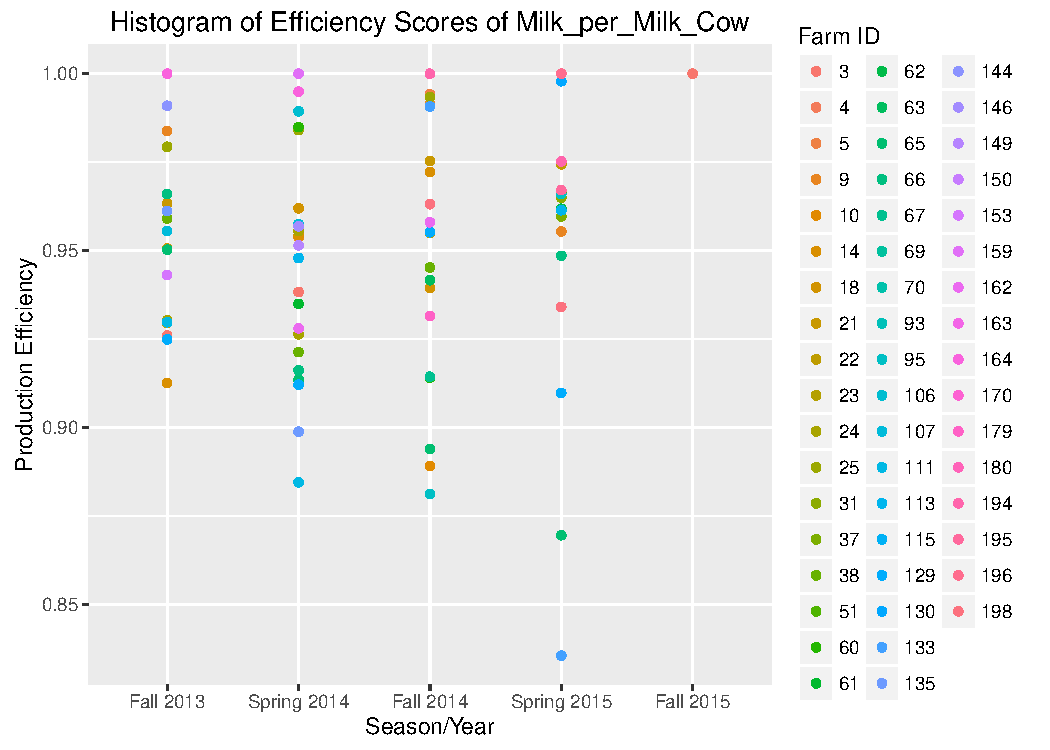
\includegraphics{Final_Model-009}
\caption{Test Data Efficiency Score over Time (output: Milk)}
\end{figure}

\begin{figure}[H]
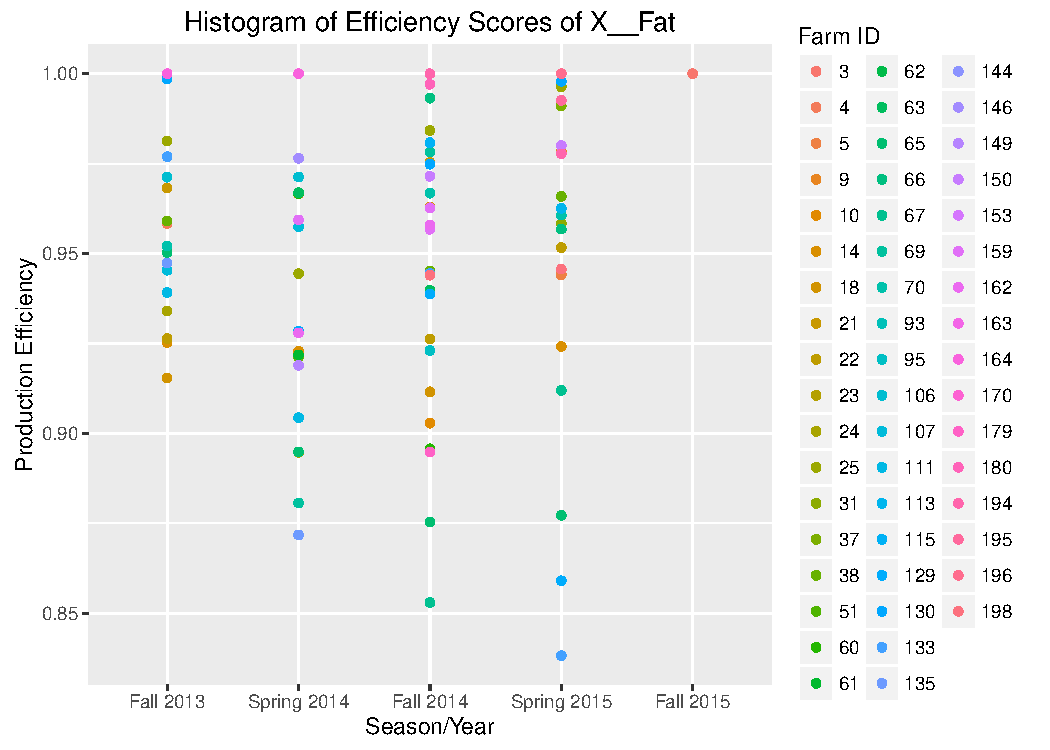
\includegraphics{Final_Model-010}
\caption{Test Data Efficiency Score over Time (output: Fat)}
\end{figure}
\begin{figure}[H]
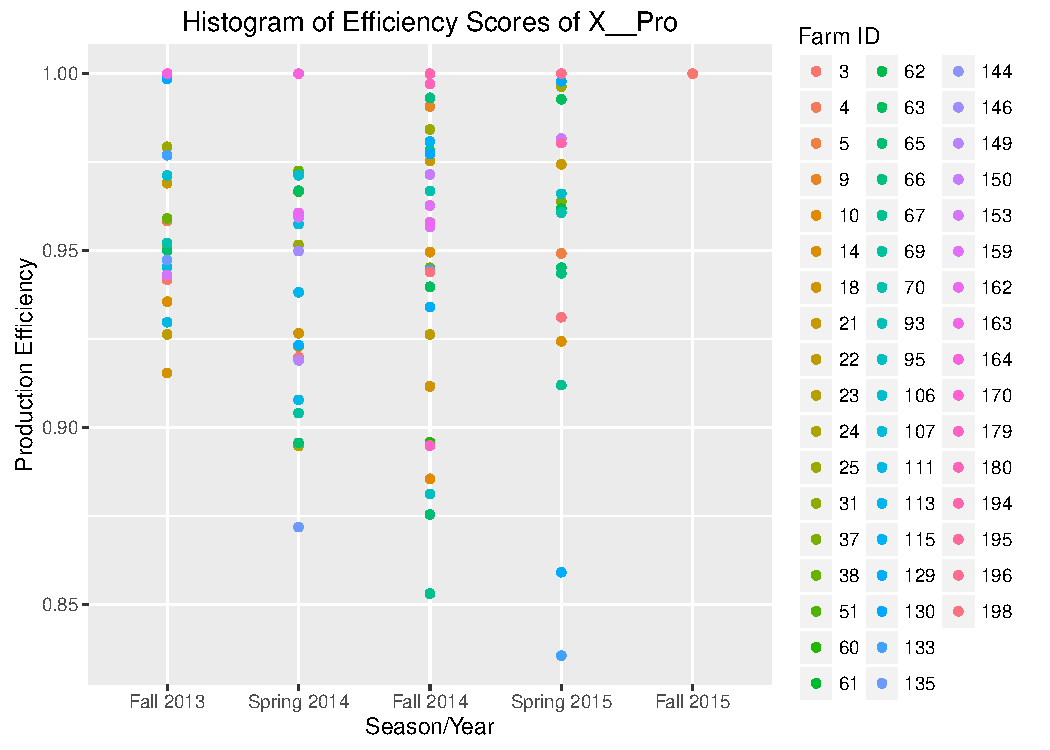
\includegraphics{Final_Model-011}
\caption{Test Data Efficiency Score over Time (output: Protein)}
\end{figure}
\begin{figure}[H]
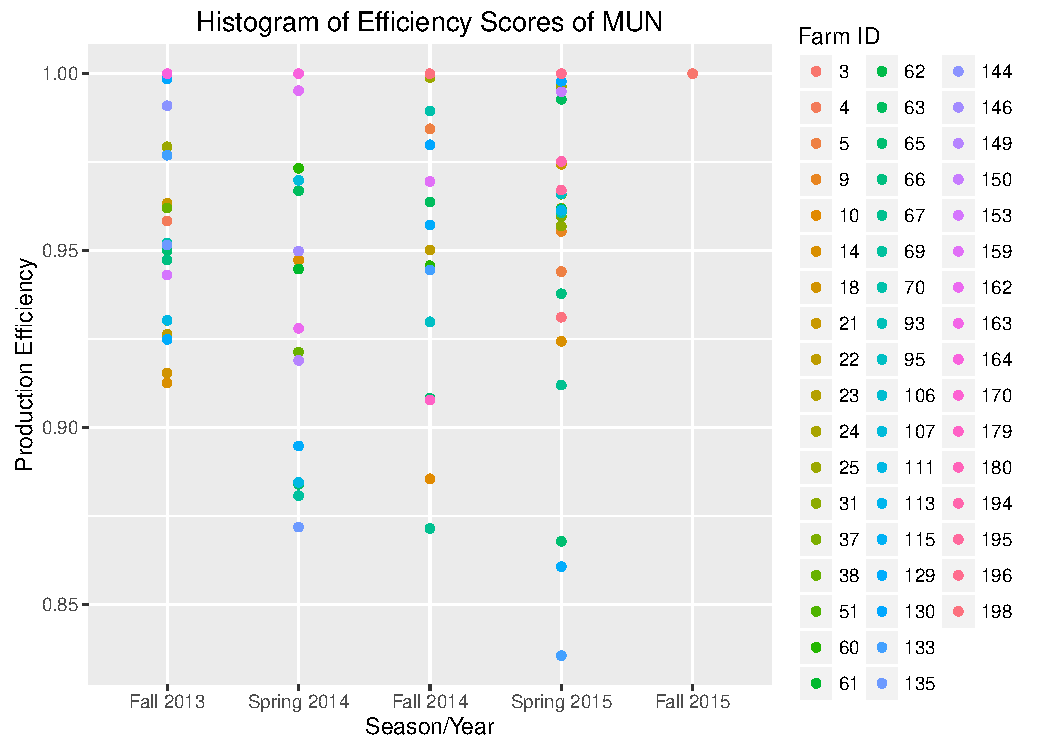
\includegraphics{Final_Model-012}
\caption{Test Data Efficiency Score over Time (output: MUN)}
\end{figure}
\begin{figure}[H]
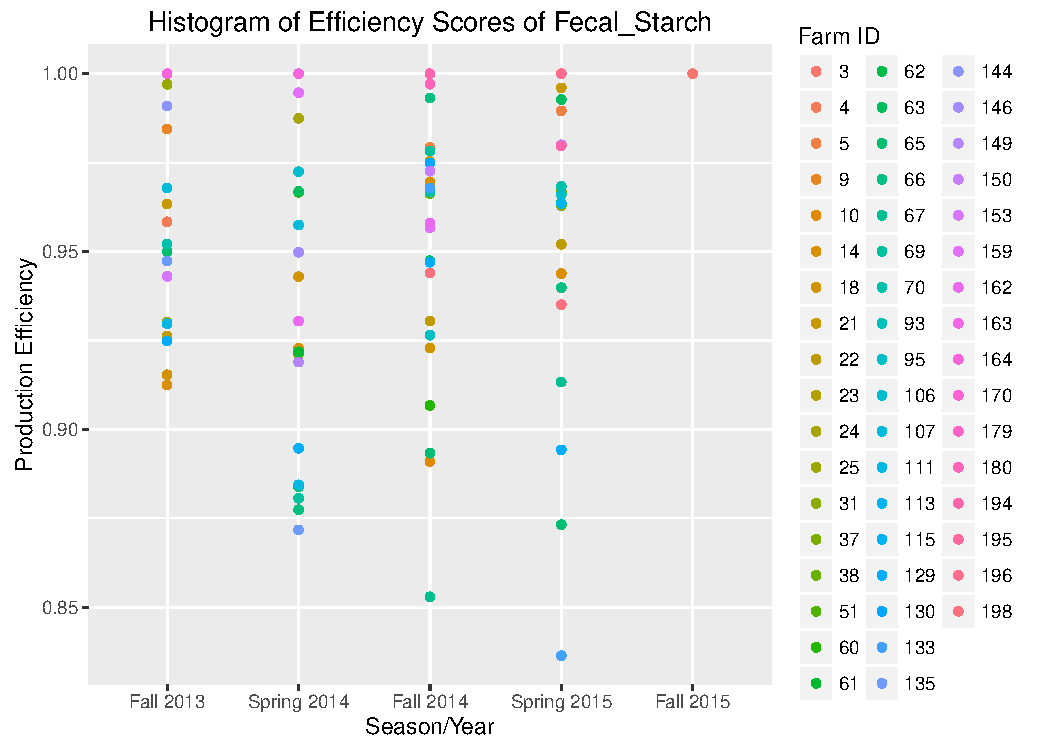
\includegraphics{Final_Model-013}
\caption{Test Data Efficiency Score over Time (output: Fecal Starch)}
\end{figure}

\subsection{Model 5 Annual Data}
In this section, we merge annual data into pooled test date data. We have 55 avaible observations in total. With annual data, we are able to use Purchased Feed, Feed Cost, Corn silage as input variables. For each of these output variables, we conduct DEA for all farms. The average efficiency scores can be summarized in table 4.

% latex table generated in R 3.2.2 by xtable 1.8-2 package
% Fri Apr 01 23:40:09 2016
\begin{longtable}{l|l|l|l|l|l|l}
  \hline
 & Farm\_ID & Milk\_per\_Milk\_Cow & X\_\_Fat & X\_\_Pro & MUN & Fecal\_Starch \\ 
  \hline
1 & 3.00 & 0.94 & 0.93 & 0.93 & 0.93 & 0.93 \\ 
  2 & 4.00 & 1.00 & 1.00 & 1.00 & 1.00 & 1.00 \\ 
  3 & 5.00 & 1.00 & 1.00 & 1.00 & 1.00 & 1.00 \\ 
  4 & 9.00 & 1.00 & 1.00 & 1.00 & 1.00 & 1.00 \\ 
  5 & 10.00 & 0.89 & 0.90 & 0.94 & 0.89 & 0.89 \\ 
  6 & 14.00 & 0.96 & 0.95 & 0.95 & 0.97 & 0.96 \\ 
  7 & 18.00 & 0.99 & 0.98 & 0.98 & 0.98 & 0.98 \\ 
  8 & 21.00 & 0.99 & 1.00 & 1.00 & 1.00 & 0.99 \\ 
  9 & 22.00 & 0.98 & 0.97 & 0.97 & 0.97 & 0.97 \\ 
  10 & 23.00 & 1.00 & 1.00 & 1.00 & 1.00 & 1.00 \\ 
  11 & 24.00 & 0.94 & 0.93 & 0.93 & 0.93 & 0.96 \\ 
  12 & 25.00 & 0.99 & 0.97 & 0.98 & 0.99 & 1.00 \\ 
  13 & 37.00 & 1.00 & 1.00 & 1.00 & 1.00 & 1.00 \\ 
  14 & 38.00 & 0.98 & 0.98 & 0.98 & 0.99 & 0.99 \\ 
  15 & 63.00 & 1.00 & 1.00 & 1.00 & 1.00 & 1.00 \\ 
  16 & 65.00 & 1.00 & 1.00 & 1.00 & 1.00 & 1.00 \\ 
  17 & 66.00 & 0.93 & 0.92 & 0.93 & 0.95 & 0.93 \\ 
  18 & 67.00 & 1.00 & 1.00 & 1.00 & 1.00 & 1.00 \\ 
  19 & 69.00 & 0.98 & 0.95 & 0.95 & 0.95 & 0.95 \\ 
  20 & 70.00 & 0.99 & 0.99 & 1.00 & 0.99 & 0.99 \\ 
  21 & 106.00 & 1.00 & 0.99 & 0.99 & 0.99 & 1.00 \\ 
  22 & 107.00 & 1.00 & 1.00 & 1.00 & 1.00 & 1.00 \\ 
  23 & 113.00 & 0.99 & 0.98 & 0.98 & 0.98 & 1.00 \\ 
  24 & 129.00 & 0.96 & 0.97 & 0.98 & 0.96 & 0.96 \\ 
  25 & 130.00 & 1.00 & 0.99 & 0.99 & 0.99 & 0.99 \\ 
  26 & 133.00 & 1.00 & 0.95 & 0.95 & 0.95 & 0.98 \\ 
  27 & 135.00 & 0.90 & 0.89 & 0.89 & 0.89 & 0.90 \\ 
  28 & 146.00 & 1.00 & 1.00 & 1.00 & 1.00 & 1.00 \\ 
  29 & 149.00 & 0.95 & 0.93 & 0.93 & 0.93 & 0.95 \\ 
  30 & 159.00 & 1.00 & 0.95 & 0.95 & 0.95 & 0.98 \\ 
  31 & 162.00 & 0.99 & 0.99 & 1.00 & 0.99 & 0.99 \\ 
   \hline
\hline
\caption{Average Annual Data Efficiency Score by Farm} 
\label{Table-4}
\end{longtable}Each column is table 4 reports the average efficiency score based on that column as output. We plot the distribution of the efficiency scores in figure 8 and figure 9.

\begin{figure}[H]
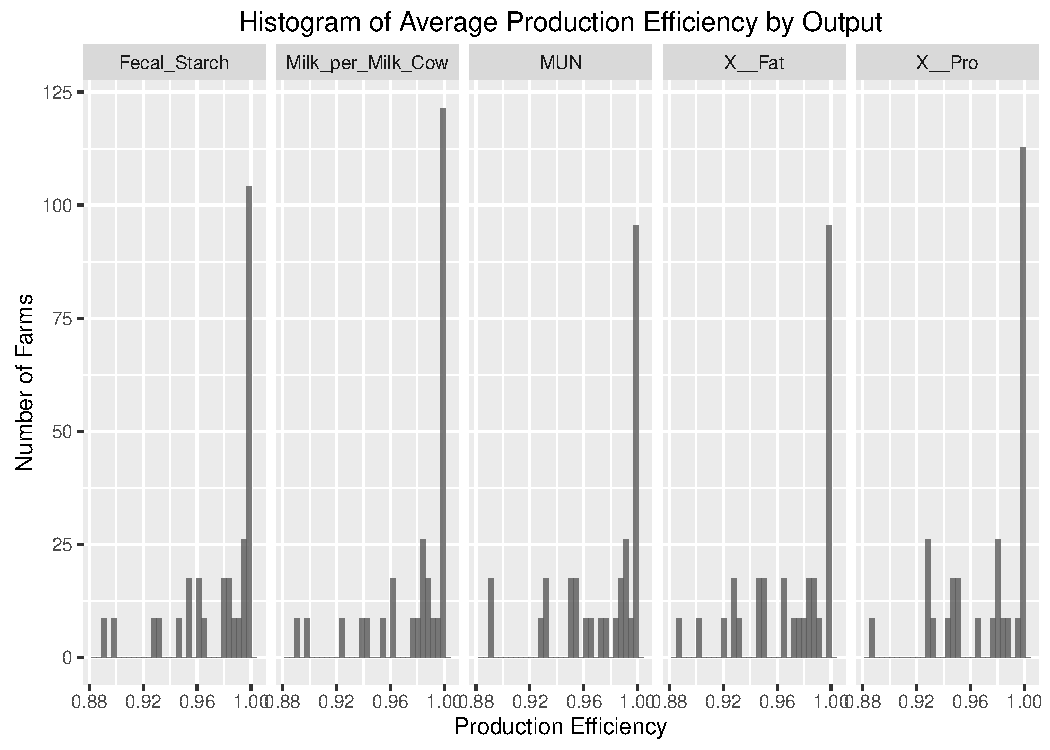
\includegraphics{Final_Model-33}
\caption{Histogram of Average Efficiency Score for each farm}
\end{figure}


\begin{figure}[H]
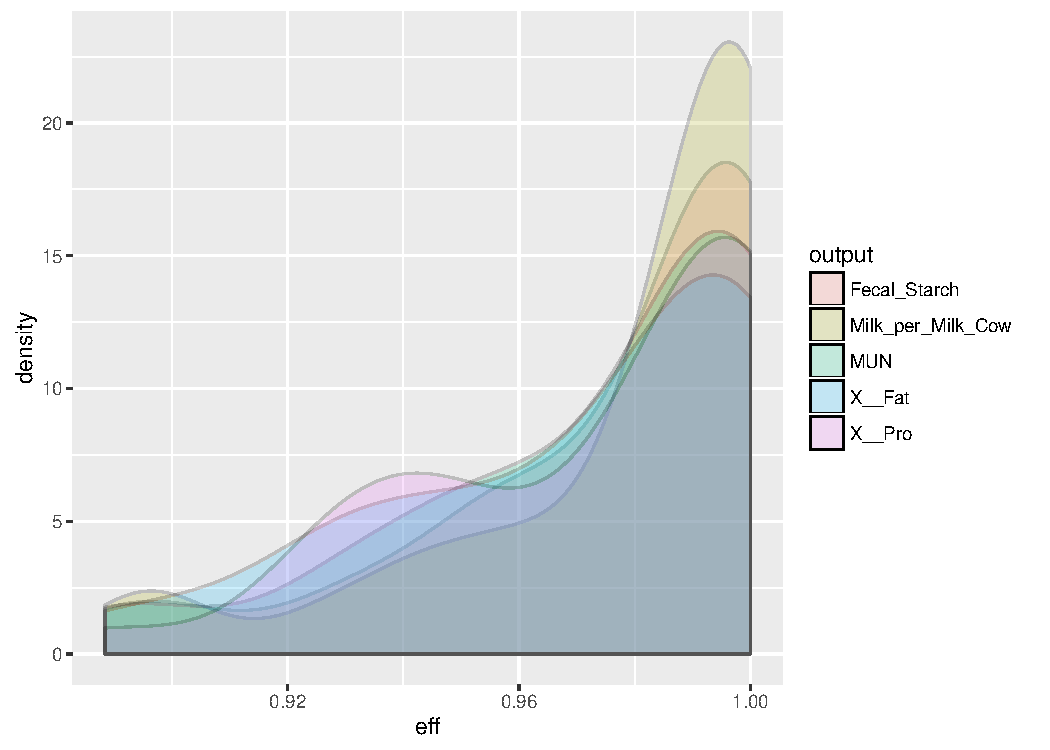
\includegraphics{Final_Model-44}
\caption{Distribution of Average Efficiency Score for each farm}
\end{figure}

\section{New Addition 03/31/2016}
\subsection{Plot efficiency versus Variates}
In this section we plot the efficiency score we got in section 2.1 (Model 4-1) versus fecal starch, starch digestibility, and MUN.

\begin{figure}[H]
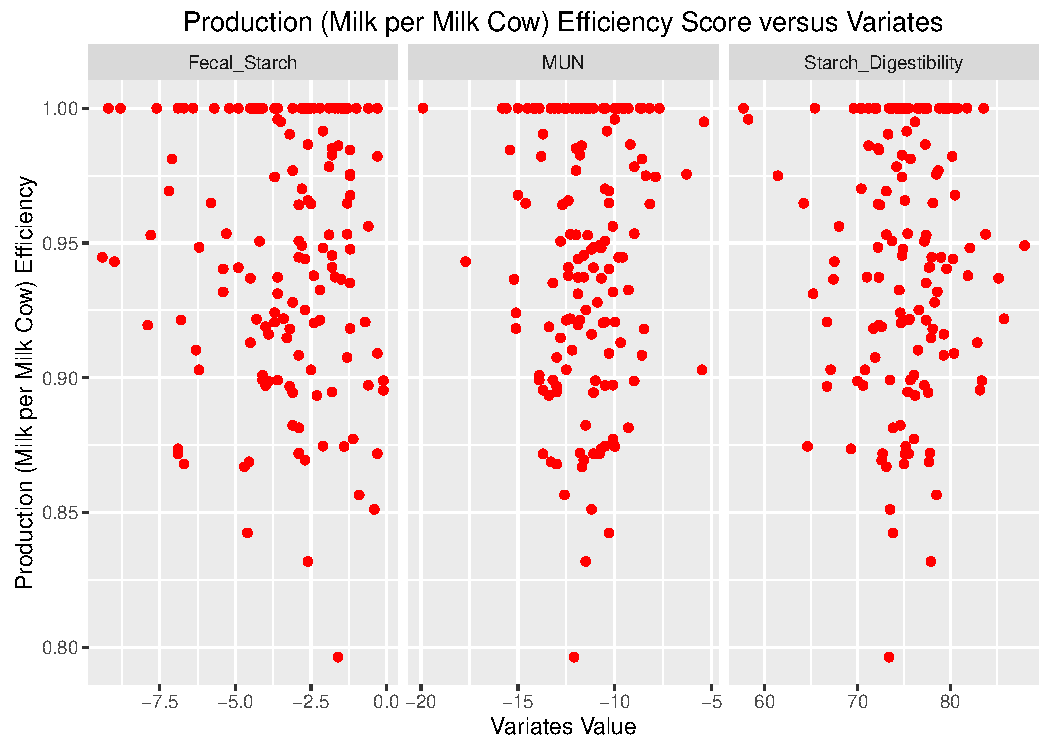
\includegraphics{Final_Model-03312016_1}
\caption{Production (Milk per Milk Cow) Efficiency Score versus Variates}
\end{figure}

\begin{figure}[H]
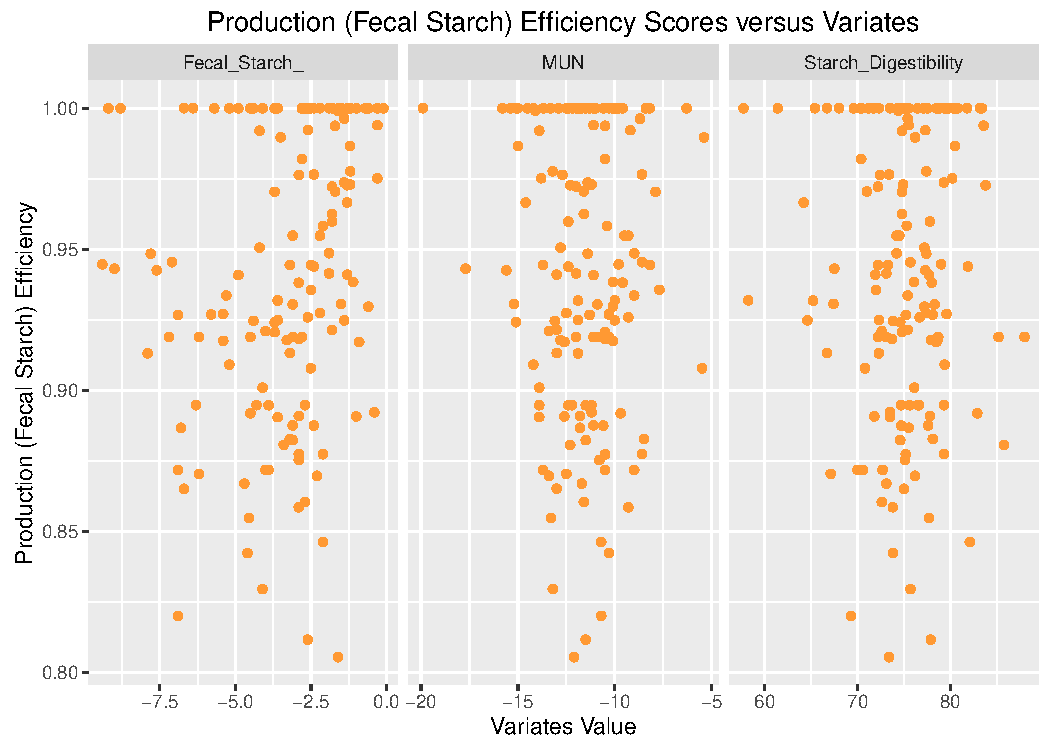
\includegraphics{Final_Model-03312016_2}
\caption{Production (Fecal Starch) Efficiency Scores versus Variates}
\end{figure}



\subsection{Plot efficiency versus Variates by Group (0-100 cows, 100-275 cows)}

\begin{figure}[H]
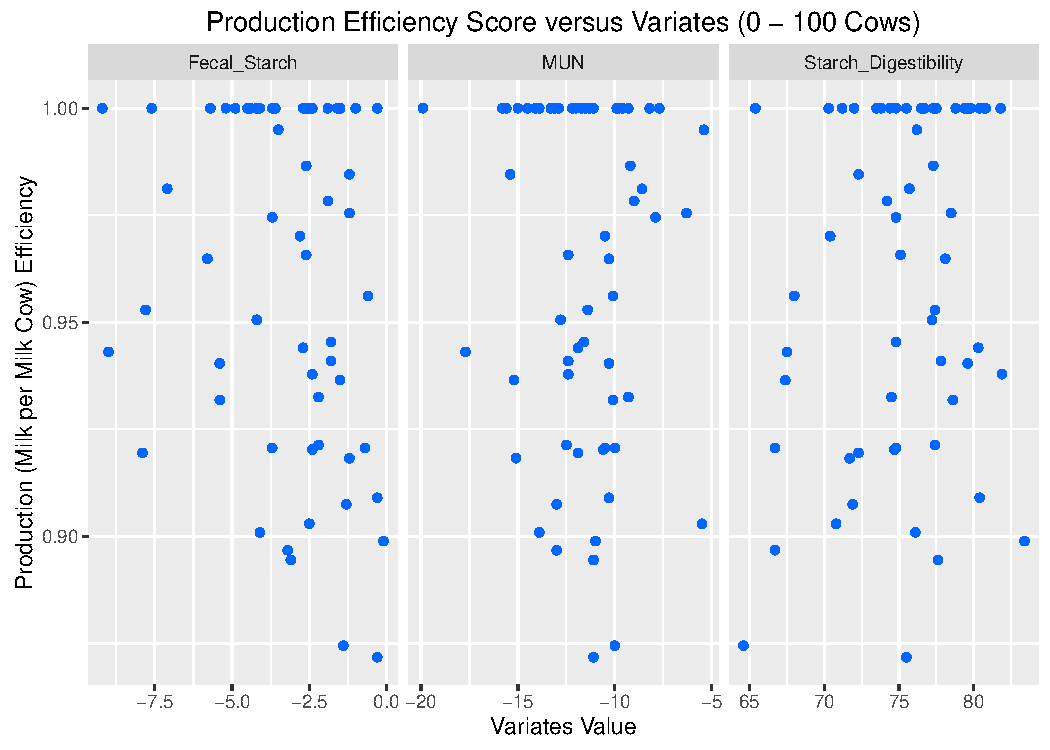
\includegraphics{Final_Model-03312016_3}
\caption{Production Efficiency Score versus Variates (0 - 100 Cows)}
\end{figure}

\begin{figure}[H]
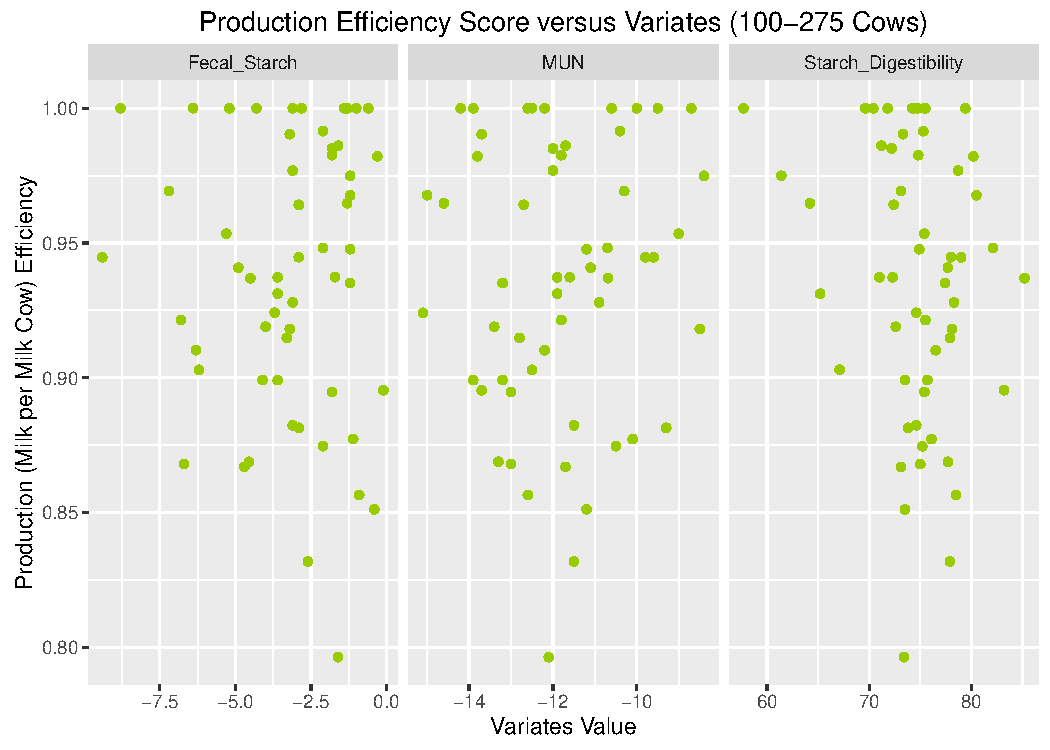
\includegraphics{Final_Model-03312016_4}
\caption{Production Efficiency Score versus Variates (100-275 Cows)}
\end{figure}


\subsection{Two-Step DEA}
In this section we run two step DEA on the Annual Data.
\textbf{Step 1}: For the whole data, we estimate efficiency score using DEA.
\textbf{Step 2}: We run a tobit regression of efficiency score on four variates (daily IOFC Surplus Group, Crop Cost, Purchased Feed and Corn Silage). The results are as follows.
\begin{Schunk}
\begin{Soutput}
Call:
censReg(formula = Annual_eff$eff_Milk_per_Milk_Cow ~ Annual_eff$Pur_Feed_Calc + 
    Annual_eff$Corn_silage + Annual_eff$Fecal_Starch + Annual_eff$MUN, 
    left = 0, right = 1)

Observations:
         Total  Left-censored     Uncensored Right-censored 
            55              0             23             32 

Coefficients:
                           Estimate Std. error t value Pr(> t)    
(Intercept)               1.0082852  0.0686582  14.686  <2e-16 ***
Annual_eff$Pur_Feed_Calc  0.0012297  0.0049023   0.251  0.8019    
Annual_eff$Corn_silage   -0.0012545  0.0007313  -1.715  0.0863 .  
Annual_eff$Fecal_Starch   0.0030734  0.0043589   0.705  0.4808    
Annual_eff$MUN           -0.0064460  0.0045548  -1.415  0.1570    
logSigma                 -2.9976705  0.1673256 -17.915  <2e-16 ***
---
Signif. codes:  0 '***' 0.001 '**' 0.01 '*' 0.05 '.' 0.1 ' ' 1

Newton-Raphson maximisation, 13 iterations
Return code 2: successive function values within tolerance limit
Log-likelihood: 17.87233 on 6 Df
\end{Soutput}
\end{Schunk}

The coefficients of the tobit regression are:
\begin{Schunk}
\begin{Soutput}
             (Intercept) Annual_eff$Pur_Feed_Calc   Annual_eff$Corn_silage 
             1.008285189              0.001229718             -0.001254456 
 Annual_eff$Fecal_Starch           Annual_eff$MUN                 logSigma 
             0.003073360             -0.006445951             -2.997670468 
\end{Soutput}
\end{Schunk}

The marginal effects $\frac{\partial \mathbbm{E}(Y|X)}{\partial x_j}$ are
\begin{Schunk}
\begin{Soutput}
Annual_eff$Pur_Feed_Calc   Annual_eff$Corn_silage  Annual_eff$Fecal_Starch 
            0.0005122647            -0.0005225698             0.0012802721 
          Annual_eff$MUN 
           -0.0026851951 
\end{Soutput}
\end{Schunk}

\end{document}
